%%%%%%%%%%%%%%%%%%%%%%%%%%%%%%%%%%%%%%%%%%%%%%%%%%%%%%%%%%%%%%%%%%
%%%%%%%% ICML 2013 EXAMPLE LATEX SUBMISSION FILE %%%%%%%%%%%%%%%%%
%%%%%%%%%%%%%%%%%%%%%%%%%%%%%%%%%%%%%%%%%%%%%%%%%%%%%%%%%%%%%%%%%%

% Use the following line _only_ if you're still using LaTeX 2.09.
%\documentstyle[icml2013,epsf,natbib]{article}
% If you rely on Latex2e packages, like most moden people use this:
\documentclass{article}

% For figures
\usepackage{graphicx} % more modern
%\usepackage{epsfig} % less modern
% \usepackage{subfigure}
\usepackage{subcaption}
\usepackage{multicol}

% For citations
\usepackage{natbib}

% For algorithms
\usepackage{algorithm}
\usepackage{algorithmic}

% For math
\usepackage{amsmath}
\usepackage{siunitx}

% As of 2011, we use the hyperref package to produce hyperlinks in the
% resulting PDF.  If this breaks your system, please commend out the
% following usepackage line and replace \usepackage{icml2013} with
% \usepackage[nohyperref]{icml2013} above.
\usepackage{hyperref}

% Packages hyperref and algorithmic misbehave sometimes.  We can fix
% this with the following command.
\newcommand{\theHalgorithm}{\arabic{algorithm}}

% Employ the following version of the ``usepackage'' statement for
% submitting the draft version of the paper for review.  This will set
% the note in the first column to ``Under review.  Do not distribute.''
\usepackage{icml2013}
% Employ this version of the ``usepackage'' statement after the paper has
% been accepted, when creating the final version.  This will set the
% note in the first column to ``Proceedings of the...''
% \usepackage[accepted]{icml2013}


% The \icmltitle you define below is probably too long as a header.
% Therefore, a short form for the running title is supplied here:
\icmltitlerunning{6.867: Homework 2}

\begin{document}

\twocolumn[
  \icmltitle{6.867: Homework 2}

  % % It is OKAY to include author information, even for blind
  % % submissions: the style file will automatically remove it for you
  % % unless you've provided the [accepted] option to the icml2013
  % % package.
  % \icmlauthor{Your Name}{email@yourdomain.edu}
  % \icmladdress{Your Fantastic Institute,
  %             314159 Pi St., Palo Alto, CA 94306 USA}
  % \icmlauthor{Your CoAuthor's Name}{email@coauthordomain.edu}
  % \icmladdress{Their Fantastic Institute,
  %             27182 Exp St., Toronto, ON M6H 2T1 CANADA}

  % You may provide any keywords that you
  % find helpful for describing your paper; these are used to populate
  % the "keywords" metadata in the PDF but will not be shown in the document
  \icmlkeywords{boring formatting information, machine learning, ICML}

  \vskip 0.3in
]

\section{Logistic regression}
In this section, we explore logistic regression with L1 and L2 regularization. We use gradient descent to compare the resulting weight vectors under different regularizers and regularization parameters, and we evaluate the effect of these choices in the context of multiple data sets.

\subsection{L2 regularization}
We first consider L2 regularization, in which the objective function to minimize is
$$E_{LR}(w, w_0) = \textsc{NLL}(w, w_0) + \lambda ||w||^2_2$$
where
$$\textsc{NLL}(w, w_0) = \sum_i \log(1 + \exp(-y^{(i)} (w x^{(i)} + w_0)))$$
and in the case of L2 regularization,
$$||w|| = |w|_2 = \sqrt{w_1^2 + ... + w_n^2}$$
Gradient descent was run with this objective function on the training dataset \texttt{data1\_train.csv} with $\lambda = 0$. We observed how the weight vector changed as a function of the number of iterations of gradient descent across various initial guesses, step sizes, and convergence criterion. There were three key findings that we were able to make. First, we saw that the ultimate convergence weight was heavily dependent on the initial guess. This actually makes a good deal of sense because of the fact that there are infinitely many ways to perfectly separate a dataset that's linearly separable. The second observation was that $w_{0}$ and $w_{1}$ always decreased as number of iterations increased whereas $w_{2}$ also increased. Finally, we saw that the convergence weight values were all within the same order of magnitude as the initial guess. This makes intuitive sense since we know from class that in the case of linearly separable data, the optimization aims to make the weights as large as possible. \\

When $\lambda = 1$, we see drastically different behavior in how the weight vector changes throughout the course of the gradient descent. The primary difference is the fact that $w_{0}, w_{1}, and w_{2}$ all converge to much smaller values. For example, when we set the initial guesses to be $100$ for all 3 components of the weight vector, the converged weights were two orders of magnitude less than the initial guesses. The reason for this phenomenon is due to the regularization penalty incurred when we set $\lambda = 1$

\subsection{L1 regularization}
In the case of L1 regularization, the objective function is the same except that $||w^2_2||$ becomes replaced with $||w_1||$, whereby $||w_1||$ is defined by:
$$|w| = |w|_1 = \sum_{i=1}^n |w_i|$$
We can evaluate the different regularization techniques under different values of $\lambda$ in the context of the weight vectors, the decision boundary, and the classification error rate in each of the training data sets. Before we dive into details, we make the obvious observation that when $\lambda = 0$, the choice of regularizer ($L_1$ vs. $L_2$) makes no difference on anything since the entire term is just $0$.

\subsubsection{Weight vector}
In terms of the weight vector, we discovered that depending on whether the particular $|w_n|$ was less than or greater to $1$ either the L1 regularization resulted in a higher magnitude weight or the L2 regularization resulted in a higher magnitude weight. Specifically, when $w_n$ was less than 1, L2 regularization resulted in a higher magnitude weight, while when $w_n$ was greater than 1, L1 regularization resulted in a higher magnitude weight.   This makes intuitive sense because squaring number larger than 1 results in larger numbers while squaring numbers less than 1 result in smaller numbers. We also discovered that a larger $\lambda$ values resulted in smaller weight magnitudes for both L1 and L2.

\subsubsection{Decision boundary}
The decision boundary was able to perfectly separate the data for all values of $\lambda$ as well as for both L1 and L2 regularization when the dataset is linearly separable. Generally, all the decision boundaries looked very similar to one another across values of $\lambda$ as well as for both L1 and L2 regularization. The one slight difference we noticed is that when $\lambda = 0$ it appeared the algorithm purely tried to correctly classify the most amount of points which resulted in lines that seemed extremely close to a certain distribution while when $\lambda =1$ the algorithm seemed to be a bit better in taking in to consideration the weights of the various points which resulted in lines that seemed divide the clusters more evenly.

\subsubsection{Classification error rate}
The classification error rate is always $0$ for all values of $\lambda$ as well as for both L1 and L2 regularization when the dataset is linearly separable. For datasets that were non-linearly separable we found that a larger $\lambda$ generally resulted in slightly worse performance for the training sets (for example 0.9875 with $\lambda = 0$ and 0.965 with $\lambda = 1$ for training dataset 2 using L1 regularization.

\subsection{Optimization}
By using the training and validation data sets, we can identify the best regularizer and value for $\lambda$ for each of the four data sets. These results are presented in Table 1 (above). Graphs of the decision boundaries for the optimal regularizers and $\lambda$s are shown below.

\begin{table}
  \begin{center}
    \begin{tabular}{ | c | c | c | c | }
      \hline
      Data & Best regularizer & Best $\lambda$ & Test performance \\ \hline
      1       & both           & all            & 1.0 \\ \hline
      2       & both           & all            & 0.805 \\ \hline
      3       & L2               & 1             & 0.97 \\ \hline
      4       & L1               & 1             & 0.5 \\ \hline
    \end{tabular}
  \end{center}
  \caption{Optimal regularizer and $\lambda$ for datasets}
\end{table}

\begin{figure}[width=\linewidth]
\centering
\begin{multicols}{2}
  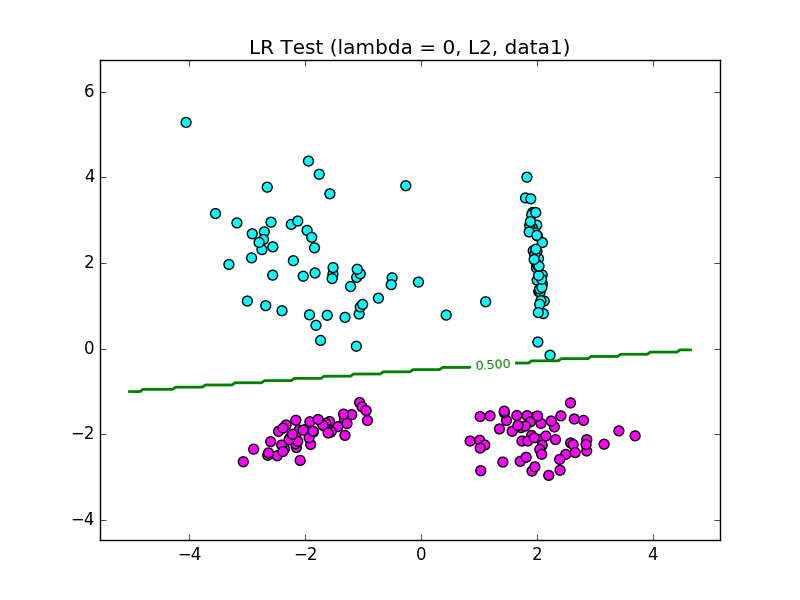
\includegraphics[width=1.2\linewidth]{Part1_data1_test.png}
  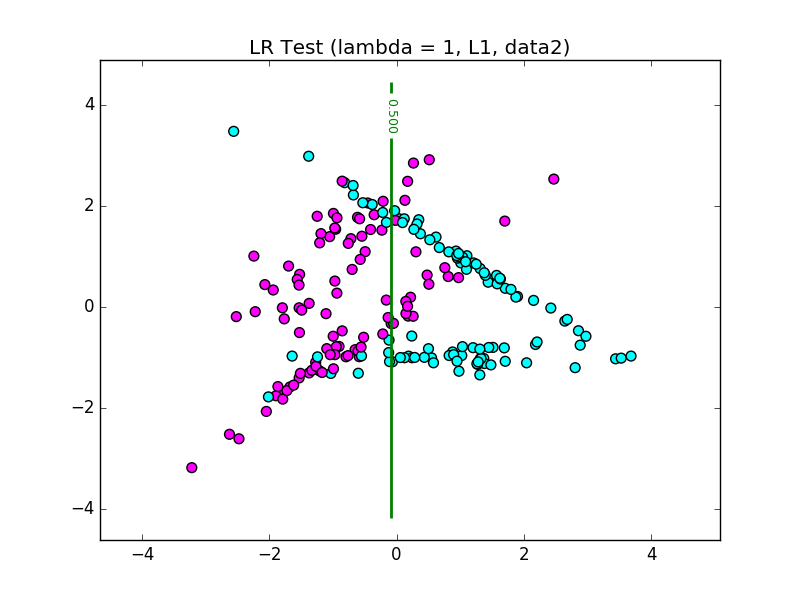
\includegraphics[width=1.2\linewidth]{Part1_data2_test.png}
  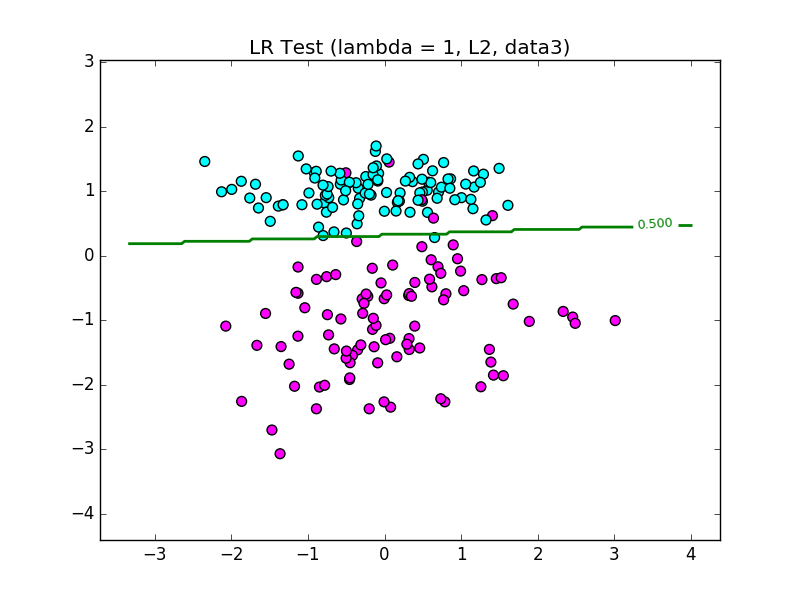
\includegraphics[width=1.2\linewidth]{Part1_data3_test.png}
  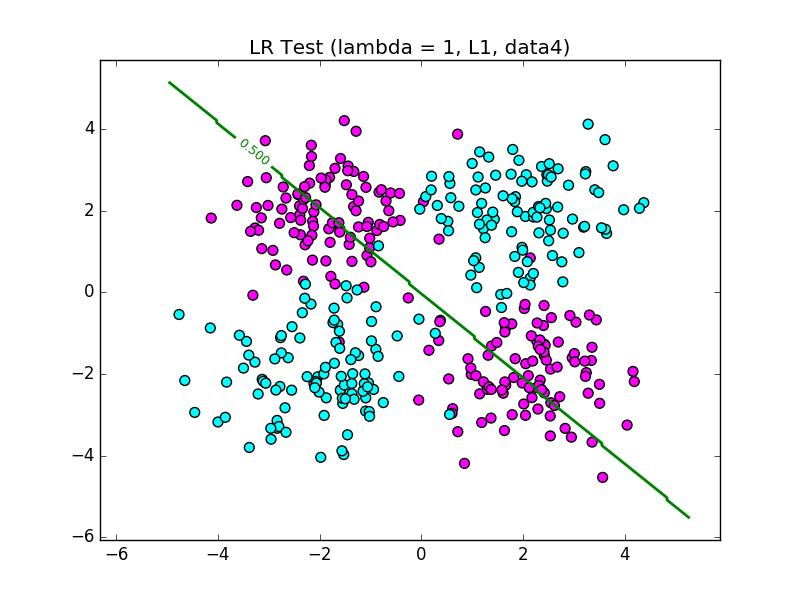
\includegraphics[width=1.2\linewidth]{Part1_data4_test.png}
\end{multicols}
\caption{decision boundaries for test data}
\end{figure}


\section{Support Vector Machine}
In this section, we explore various versions of the dual form of support vector machines, first with slack variables and then with generalized kernel functions.

\subsection{Dual form with slack variables}
We here implement a dual form of linear SVMs with slack variables. More specifically, we solve the following optimization problem with respect to $\alpha$:
$$\max_\alpha -\frac{1}{2}|\sum_i \alpha_i y^{(i)} x^{(i)}|^2 + \sum_i \alpha_i$$
$$\text{s.t.} \sum_i \alpha_i y^{(i)} = 0$$
$$0 \leq \alpha_i \leq C, 1 \leq i \leq n$$
Written another way, this maximization problem can be framed as a minimization problem:
$$\min_\alpha \frac{1}{2} x^T P x + q^T x$$
$$\text{s.t.} G x \leq h$$
$$ Ax = b $$
where $b=0$ and
$$x=
\begin{bmatrix}
  \alpha_0 \\
  \alpha_1 \\
  \vdots      \\
  \alpha_n \\
\end{bmatrix},
q=
\begin{bmatrix}
  -1 \\
  -1 \\
  \vdots \\
  -1 \\
\end{bmatrix},
A^T=
\begin{bmatrix}
  y_0 \\
  y_1 \\
  \vdots \\
  y_{n-1} \\
\end{bmatrix},
G=
\begin{bmatrix}
  I \\
  -I \\
\end{bmatrix},
$$
where $I$ and $-I$ are the identity and negative identity matrix respectively. Furthermore,
$$
P=
\begin{bmatrix}
  x_0^2 y_0^2             & x_0 y_0 x_1 y_1         & \dots  & x_0 y_0 x_{n-1} y_{n-1}\\
  x_1 y_1 x_0 y_0         & x_1^2 y_1^2             & \dots  & x_1 y_1 x_{n-1} y_{n-1}\\
  \vdots                  & \vdots                  & \ddots & \vdots \\
  x_{n-1} y_{n-1} x_0 y_0 & x_{n-1} y_{n-1} x_1 y_1 & \dots  & x_{n-1}^2 y_{n-1}^2\\
\end{bmatrix}
$$
$$
h^T=
\begin{bmatrix}
  C & \dots & C & 0 & \dots & 0 \\
\end{bmatrix}
$$
In the context of the four-point 2D problem, we seek to solve the following optimization:
$$\min_\alpha \frac{1}{2}
\begin{bmatrix}
  \alpha_0 \\
  \alpha_1 \\
  \alpha_2 \\
  \alpha_3 \\
\end{bmatrix}^T
\begin{bmatrix}
  16 & 24 & 0 & 24 \\
  24 & 36 & 0 & 36 \\
  0  & 0  & 0 & 0 \\
  24 & 36 & 0 & 36 \\
\end{bmatrix}
\begin{bmatrix}
  \alpha_0 \\
  \alpha_1 \\
  \alpha_2 \\
  \alpha_3 \\
\end{bmatrix}
+
\begin{bmatrix}
  -1 \\
  -1 \\
  -1 \\
  -1 \\
\end{bmatrix}^T
\begin{bmatrix}
  \alpha_0 \\
  \alpha_1 \\
  \alpha_2 \\
  \alpha_3 \\
\end{bmatrix}
$$
$$\text{s.t.}
\begin{bmatrix}
  1 & 0 & 0 & 0 \\
  0 & 1 & 0 & 0 \\
  0 & 0 & 1 & 0 \\
  0 & 0 & 0 & 1 \\
  -1 & 0 & 0 & 0 \\
  0 & -1 & 0 & 0 \\
  0 & 0 & -1 & 0 \\
  0 & 0 & 0 & -1 \\
\end{bmatrix}
\begin{bmatrix}
  \alpha_0 \\
  \alpha_1 \\
  \alpha_2 \\
  \alpha_3 \\
\end{bmatrix}
\leq
\begin{bmatrix}
  C \\
  C \\
  C \\
  C \\
  0 \\
  0 \\
  0 \\
  0 \\
\end{bmatrix},
\begin{bmatrix}
  2 \\
  3 \\
  -1 \\
  -2 \\
\end{bmatrix}
\begin{bmatrix}
  \alpha_0 \\
  \alpha_1 \\
  \alpha_2 \\
  \alpha_3 \\
\end{bmatrix}
= 0 $$

Solving for $x$ when $C=1$, we get that $
\begin{bmatrix}
  \alpha_0 & \alpha_1 & \alpha_2 & \alpha_3
\end{bmatrix}^T
=
\begin{bmatrix}
  0.1875 & 0 & 0.3750 & 0 &
\end{bmatrix}^T
$. This indicates that the first and third samples are support vectors because $0 \leq \alpha_i \leq C$. \\

Our implementation of the dual form of SVMs with slack variables was run on each of the four 2D datasets provided. With $C=1$, the decision boundaries and classification error rates were determined. This information is illustrated and summarized in Figure 2 and Table 2, respectively. As can be seen from the classification error rates in training and validation, depending on the values of the trained parameters and the spread of the datasets, the classification error could be greater for the training data (as in dataset 2), for the validation data (as in dataset 4), or equal (as in dataset 1). \\

It is interesting to note that due to numerical rounding and errors, the $\alpha$ values obtained were not exactly equal to 0 or $C$, but instead usually varied by a small threshold. In our case, we chose a threshold of $0.00001$ in order to filter out $\alpha$ values extremely close to 0 or $C$ and select for "true" support vectors. Varying this threshold however could change the classification of data as support vectors or not, and this could ultimately affect the accuracy and error rate of our classifier.

\begin{figure}[width=\linewidth]
\centering
\begin{multicols}{2}
  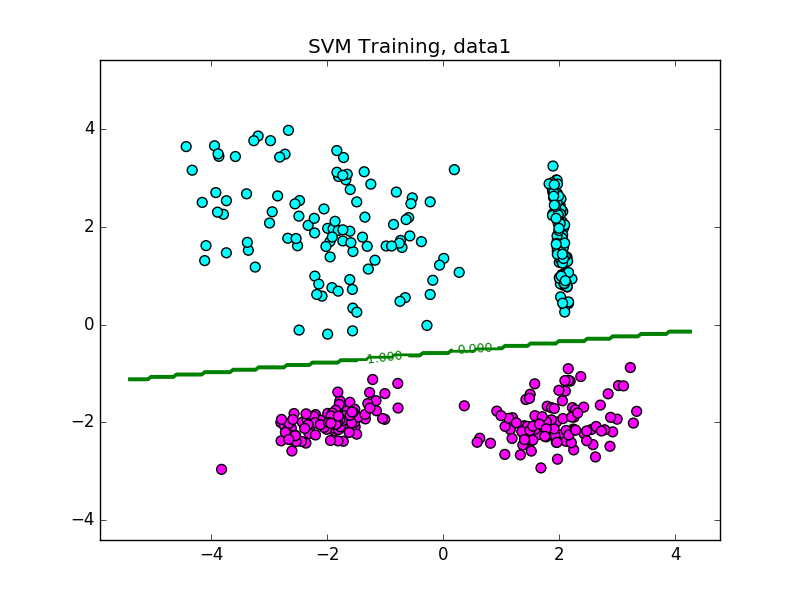
\includegraphics[width=1.2\linewidth]{code/P2/data1,training.png}
  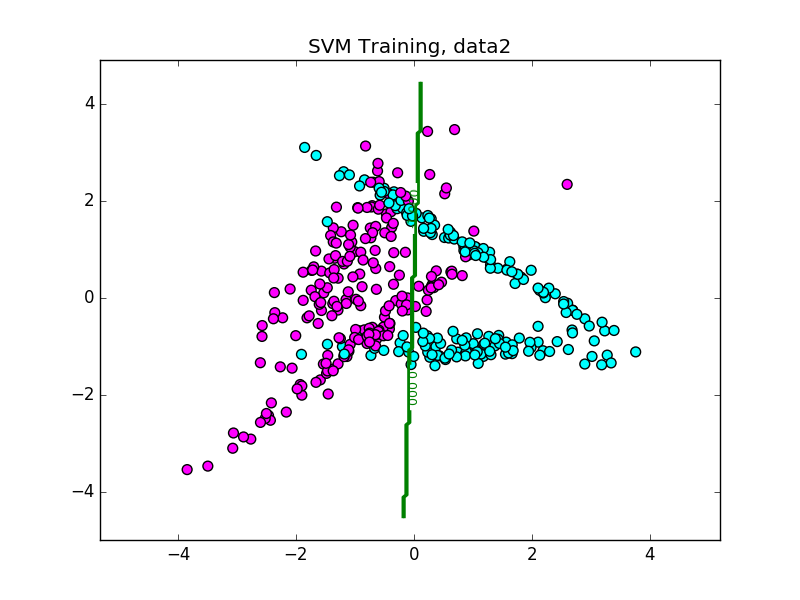
\includegraphics[width=1.2\linewidth]{code/P2/data2,training.png}
  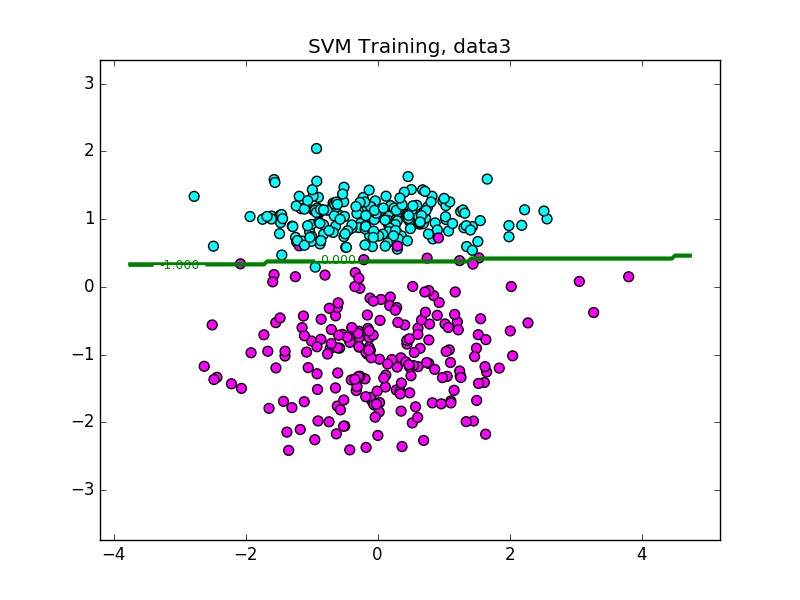
\includegraphics[width=1.2\linewidth]{code/P2/data3,training.png}
  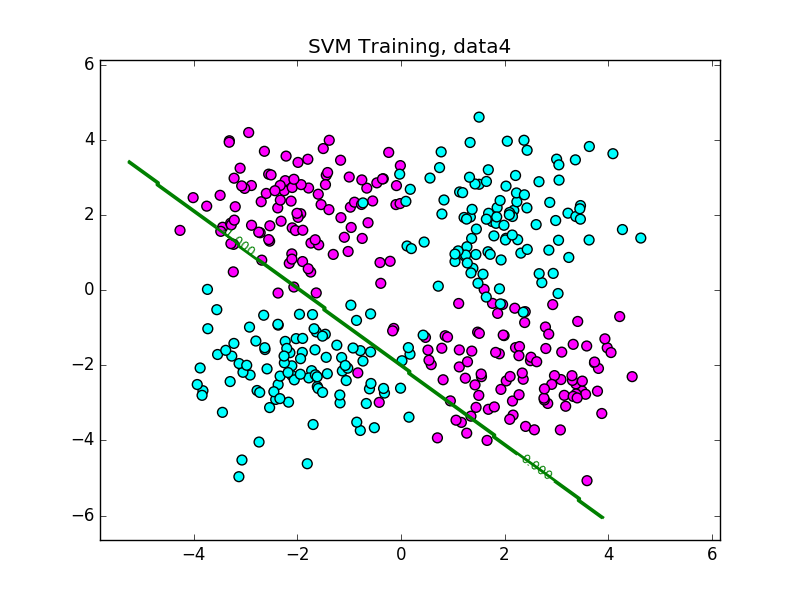
\includegraphics[width=1.2\linewidth]{code/P2/data4,training.png}
  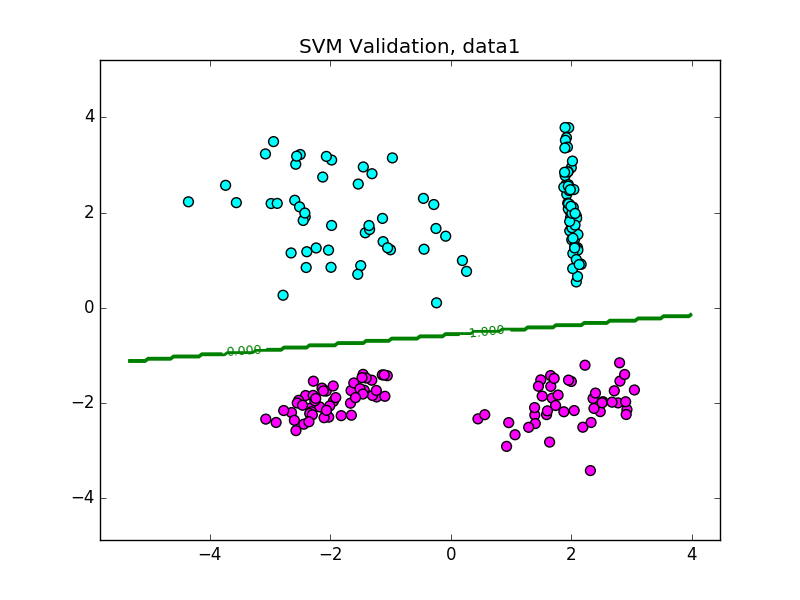
\includegraphics[width=1.2\linewidth]{code/P2/data1,validation.png}
  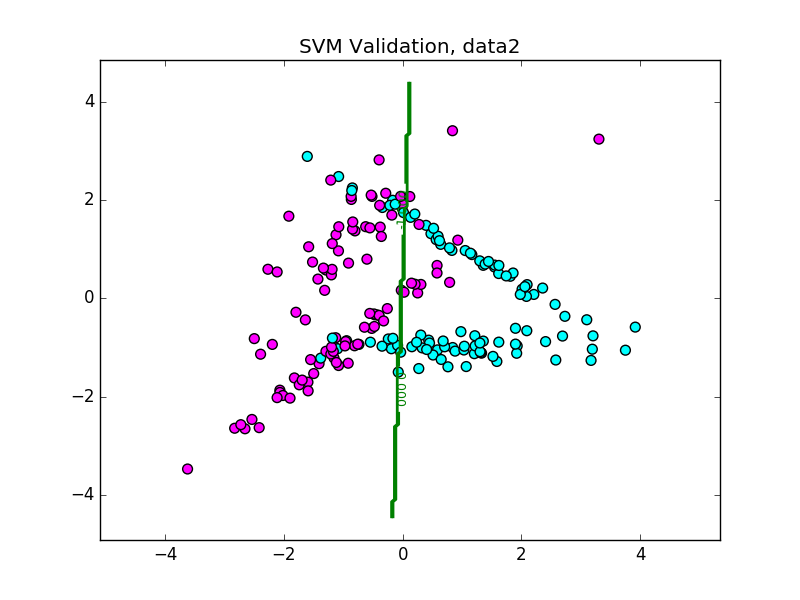
\includegraphics[width=1.2\linewidth]{code/P2/data2,validation.png}
  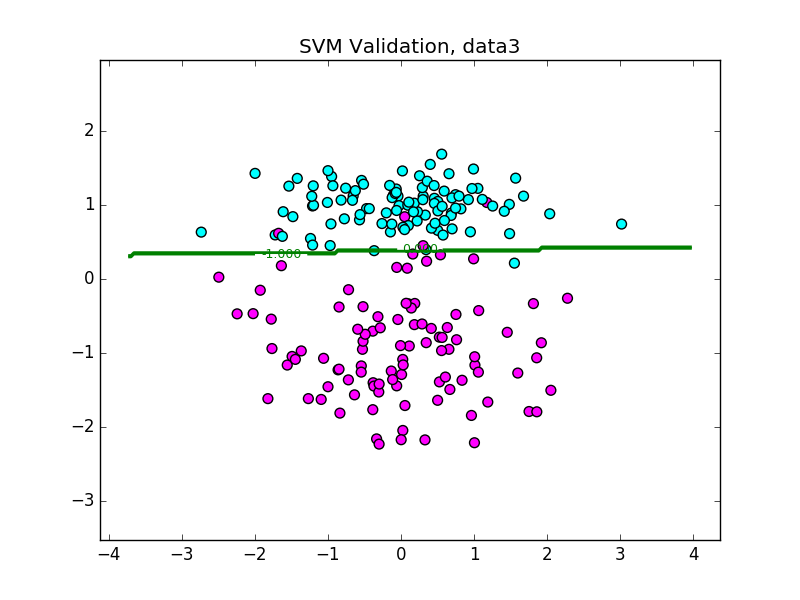
\includegraphics[width=1.2\linewidth]{code/P2/data3,validation.png}
  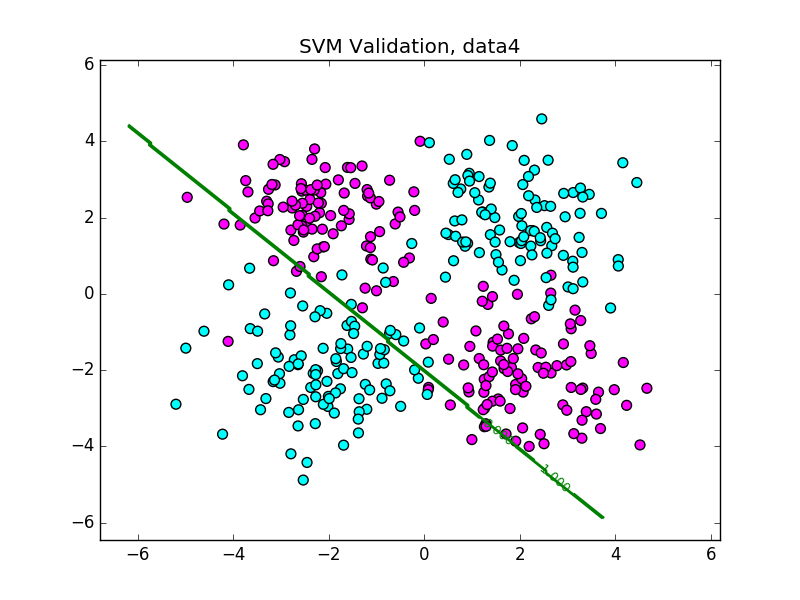
\includegraphics[width=1.2\linewidth]{code/P2/data4,validation.png}
\end{multicols}
\caption{Training and validation decision boundary}
\end{figure}

\begin{table}
  \begin{center}
    \begin{tabular}{ | c | c | c | }
      \hline
      Dataset & Training error rate & Validation error rate \\ \hline
      1       & 0.0                 & 0.0                   \\ \hline
      2       & 0.1775              & 0.09                  \\ \hline
      3       & 0.02                & 0.015                 \\ \hline
      4       & 0.3                 & 0.305                 \\ \hline
    \end{tabular}
  \end{center}
  \caption{Training and validation error rates}
\end{table}

\subsection{Dual form with kernels}
We here extend our dual form SVM to take kernel functions and kernel matrices as input. This has important implications for a number of reasons including performance and minimizing the cost of operations, as well as space and storage. We here implemented the dual form of SVMs with kernels for two kernel functions: (1) linear kernels, and (2) Gaussian radial basis function (RBF) kernels, while varying the value of $C$. \\

As the value of $C$ increased, on a conceptual level, the margin error should decrease. This is because \\ \\ \\ \\

As the value $C$ was increased, the number of support vectors generally did not show any noticeable or significant trends with a linear kernel. For all the data sets for varying values of $C$, the number of support vectors stayed roughly constant at around 3 or 4. However, for the Gaussian RBF kernel, the number of support vectors generally increased as the value of $C$ increased until a certain point (generally around $C=1$), after which the number of support vectors plateaued or even decreased. This data for the Gaussian RBF is summarized in Table 4.

\begin{table}
  \begin{center}
    \begin{tabular}{ | c | c | c | c | c | c | }
      \hline
              & $C=0.01$ & $C=0.1$ & $C=1$ & $C=10$ & $C=100$ \\ \hline
      1       & 0        & 29      & 45    & 49     & 48      \\ \hline
      2       & 0        & 21      & 32    & 32     & 36      \\ \hline
      3       & 2        & 16      & 28    & 25     & 20      \\ \hline
      4       & 0        & 35      & 79    & 78     & 75      \\ \hline
    \end{tabular}
  \end{center}
  \caption{Number of support vectors by C value}
\end{table}

\section{Pegasos}

\section{Handwritten digit recognition}



\end{document}


% This document was modified from the file originally made available by
% Pat Langley and Andrea Danyluk for ICML-2K. This version was
% created by Lise Getoor and Tobias Scheffer, it was slightly modified
% from the 2010 version by Thorsten Joachims & Johannes Fuernkranz,
% slightly modified from the 2009 version by Kiri Wagstaff and
% Sam Roweis's 2008 version, which is slightly modified from
% Prasad Tadepalli's 2007 version which is a lightly
% changed version of the previous year's version by Andrew Moore,
% which was in turn edited from those of Kristian Kersting and
% Codrina Lauth. Alex Smola contributed to the algorithmic style files.
